\subsubsection{\stid{3.06} PETSc-TAO} \label{subsubsect:petsc}
\paragraph{Overview} 

Algebraic solvers (generally nonlinear solvers that use sparse linear solvers via Newton's method) and ODE/DAE 
integrators form the core computation of many numerical simulations. No scalable ``black box'' sparse solvers 
or integrators work for all applications, nor single implementations that work well for all scales of 
problem size. Hence, algebraic solver packages provide a wide variety of algorithms and implementations 
that can be customized for the application and range of problem sizes at hand. PETSc~\cite{petsc:homepage,petsc-man} 
is a widely used software library for the scalable solution of linear, nonlinear, and ODE/DAE systems and 
computation of adjoints (sometimes called sensitivities) of ODE systems. We focus on three topics: (1) partially 
matrix-free scalable solvers efficiently use many-core and GPU-based systems; (2) reduced synchronization 
algorithms that can scale to larger concurrency than solvers with synchronization points; and (3) performance 
and data structure optimizations for all the core data structures to better utilize many-core and GPU-based 
systems as well as provide scalability to the Exascale.

The availability of systems with over 100 times the processing power of today's machines compels the utilization 
of these systems not just for a single ``forward solve'' simulation (as discussed above) but rather within a 
tight loop of optimization, sensitivity analysis (SA), and uncertain quantification (UQ). This requires the 
implementation of a new, scalable library for managing a dynamic hierarchical collection of running scalable 
simulations, where the simulations directly feed results into the optimization, SA, and UQ solvers.  This library, 
which we call libEnsemble, directs the multiple concurrent ``function evaluations'' through the tight coupling 
and feedback described above. This work consist of two parts: (1) the development of libEnsemble and (2) the 
development of algorithms and software to utilize libEnsemble.

\paragraph{Key Challenges}

A key challenge for for scaling the PETSc/TAO numerical libraries to Exascale systems is that 
traditional ``sparse-matrix-based'' techniques for linear, nonlinear, and ODE solvers, as well 
as optimization algorithms, are memory-bandwidth limited.  Another difficulty is that any 
synchronizations required across all compute units--for example, an inner product or a 
norm--can dramatically affect the scaling of the solvers.

Running an ensemble of simulation requires a coordination layer that handles load balancing and
allows the collection of running simulations to grow and shrink based on feedback. Thus, this 
library must be able to dynamically start simulations with different parameters, resume 
simulations to obtain more accurate results, prune running simulations that the solvers 
determine can no longer provide useful information, monitor the progress of the simulations, 
and stop failed or hung simulations, and collect data from the individual simulations both 
while they are running and at the end.

\paragraph{Solution Strategy}

To address the scalability of the numerical libraries, we are developing new solvers and data 
structures including pipeline Krylov methods that delay the use of the results of inner products 
and norms, allowing overlapping of the reductions and other computation; partially matrix-free 
solvers using high-order methods that have high floating-point-to-memory-access ratios and
good potential to use many-core and GPU-based systems; and in-node optimizations of sparse 
matrix-matrix products needed by algebraic multigrid to better utilize many-core systems
using a thread neutral ``bypass MPI'' approach, which implements default interprocessor 
communication using MPI but bypasses the use of MPI in performance-critical regions 
for higher performance and thereby maintains MPI portability.

Our strategy for coordinating ensemble computations has been to develop libEnsemble
to satisfy our needs.  This library should not be confused with workflow-based 
scripting systems; rather it is a library that, through the tight coupling and 
feedback described above, directs the multiple concurrent ``function evaluations''
needed by optimization, SA, and UQ solvers.

\paragraph{Recent Progress}

In the past year, we have released PETSc/TAO 3.12 (available at \url{http://www.mcs.anl.gov/petsc})
that features enhanced GPU support.  Perhaps the most important is the support for CUDA-aware 
MPI, which allows direct communication of data between Summit GPUs, bypassing the previously 
needed step of first copying the data to the CPU memory. This enhancement reduces the latency 
of the communication and improves bandwidth. For example, on Summit for sparse matrix-vector 
products, this led to a speedup of 33\% on one node and a speedup of 13\% on on four nodes 
for the same size problem. Another important addition is the ability to efficiently read 
in large meshes on thousands of nodes along with support for collect use of HDF5 calls. 
With these additions, the algebraic multigrid solver GAMG is up to 12x faster at scale 
on all of Summit when using the GPUs compared to using just the CPUs.

\begin{figure}
\centering
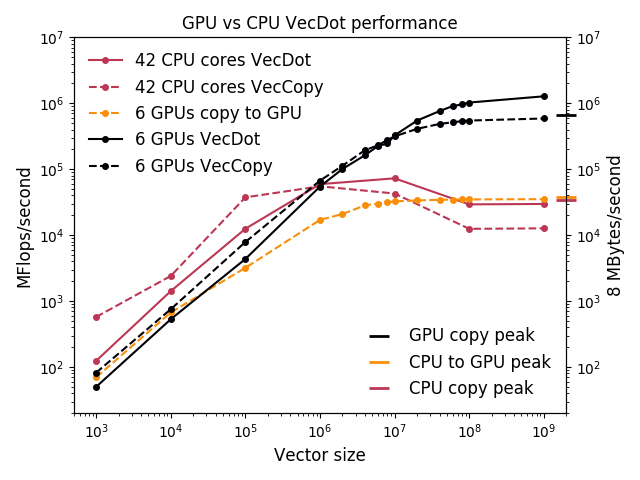
\includegraphics[width=0.5\textwidth]{projects/2.3.3-MathLibs/2.3.3.06-PETSc-TAO/petsc_profile}
\caption{Profile information on the effect of vector size on vector operations compared with 
memory throughput (one MPI rank per GPU) for PETSc/TAO 3.12. Note the log scale.}
\label{fig:petsc-tao-fig}
\end{figure}

We have also release libEnsemble 0.5.2 (available at \url{https://github.com/Libensemble/libensemble}).
Notably, this release includes several changes in progressing toward xSDK compliance had have added
support for testing on MacOS to support more applications.  We also have improved I/O, logging, 
profiling, as well as resource detection on Summit.

\paragraph{Next Steps}

Our next efforts are:
\begin{enumerate}
  \item \textbf{Enhanced application integration and performance optimization and benchmarking}:
  Refresh the AMReX/PETSc interface and ensure that the PETSc linear solvers can be used with AMReX.
  Consolidate the two MPI communication modules (VecScatter and PetscSF) to share the same code base 
  and implement two important communication optimizations in the unified code base: internode node-message 
  aggregation optimization, which is critical for scalability of GAMG, and intranode shared memory 
  optimization.  
  Ensure that libEnsemble satisfies eight of the xSDK requirements.
  Continue to produce benchmark results on Summit.
  Engage with ECP applications and co-design centers to identify new capabilities that can result in 
  FY2021-2023 application integration activities.
  \item \textbf{Harmonization, performance optimization, and software release}:
  Harmonize the quasi-Newton and line search modules between SNES and TAO to improve maintainability.
  Implement GPU optimizations of the quasi-Newton methods.
  Ensure that libEnsemble satisfies all but one of the xSDK requirements.
  Continue to produce benchmark results on Summit.
  Continue to engage with ECP applications and co-design centers.
  Release a new version of PETSc/TAO.
  \item \textbf{Enhanced application support and software release}:
  Implement and optimize the ability to use libCEED under PETSc.
  Continue to produce benchmark results on Summit.
  Continue to engage with ECP applications and co-design centers.
  Release a new version of libEnsemble that is compatible with the xSDK community policy requirements and included in the xSDK.
  \item \textbf{Benchmarking, performance optimization and software release}:
  Demonstrate new libEnsemble functionality by having libEnsemble serve as the driver/outer process that 
  invokes another xSDK tool.
  Complete benchmarking one or more of the PETSc based applications on Summit at scale including GAMG support 
  on the GPUs and identify performance bottlenecks.
  Incorporate new desired capabilities resulting from our engagement with ECP applications and co-design centers into our FY2021 plans.
  Release a new version of PETSc/TAO.
\end{enumerate}

